% This example is meant to be compiled with lualatex or xelatex
%subfigure The theme itself also supports pdflatex
\PassOptionsToPackage{unicode}{hyperref}
\documentclass[aspectratio=1610, 9pt]{beamer}

% Load packages you need here
\usepackage{polyglossia}
\setmainlanguage{german}

\usepackage{csquotes}
    

\usepackage{amsmath}
\usepackage{amssymb}
\usepackage{mathtools}

\usepackage{hyperref}
\usepackage{bookmark}

\usepackage{caption}
\usepackage{subcaption}

\usepackage[backend=biber,]{biblatex}
\addbibresource{lit.bib}

% load the theme after all packages

\usetheme[
  showtotalframes, % show total number of frames in the footline
]{tudo}

% Put settings here, like
\unimathsetup{
  math-style=ISO,
  bold-style=ISO,
  nabla=upright,
  partial=upright,
  mathrm=sym,
}

\title{LimeSurvey Tutorial}
\author[M. Maile]{Matthias Maile}
\institute[S\&K]{Sprache und Kommunikation \\ Fakultät
Rehabilitationswissenschaften}
\titlegraphic{
\includegraphics[width=0.7\textwidth]{images/tudo-title-2.jpg}}


\begin{document}

\maketitle

\begin{frame}{Lime Survey}
  \tableofcontents
\end{frame}

\begin{frame}{Kurzeinführung zu Lime Survey}
	Lime Survey ist
  \begin{itemize}
    \item Ein Tool zur Umsetzung digitaler Umfragen
    \item Ähnlich zu Google Forms
    \begin{figure}
          \centering
    	
\includegraphics[width=1.5cm]{images/forms-icon.png}
    \end{figure}
    \item \href{https://de.wikipedia.org/wiki/Free/Libre_Open_Source_Software}
	    {Freie Open Source Software}
  \end{itemize}
\end{frame}

\begin{frame}{Vorraussetzungen}
	\section{Vorraussetzungen}
	\label{sec:Vorraussetzungen}
	
	Um Lime Survey zu benutzen braucht man
  	\begin{itemize}
  	  \item Internet
	  \item Einen modernen Browser \cite{chrome-logo}\cite{firefox}
  	  \begin{figure}
  	        \centering
		\begin{subfigure}[b]{0.4\textwidth}
          		\centering
    			
\includegraphics[width=1.5cm]{images/chrome.jpeg}
		\end{subfigure}
		\begin{subfigure}[b]{0.4\textwidth}
			
\includegraphics[width=1.5cm]{images/firefox.png}
		\end{subfigure}
  	  \end{figure}
  	\item (Einen Uni Account)
		\begin{itemize}
			\item Gilt nur für das Lime Survey der TU Dortmund, also
				\url{https://umfragen.tu-dortmund.de}
		\end{itemize}
  	\end{itemize}
\end{frame}

\begin{frame}{Motivation}
	\section{Motivation}
	\label{sec:Motivation}
	
	\textbf{Warum}...
	\begin{itemize}
		\item sollten Umfragen \textbf{digital} durchgeführt werden?
		\item sollte man dafür \textbf{Lime Survey} benutzen?
	\end{itemize}
	\medskip
	Kurze Antwort: Man ist (nahezu) alternativlos:
	\begin{itemize}
		\item Google Forms
			\begin{itemize}
				\item Die Daten sind auf einem externen Server
					\\
					$\Rightarrow$ Datenschutztechnisch problematisch
				\item Man ist an Google gebunden
			\end{itemize}
		\item Klassische Papier Umfrage
			\begin{itemize}
				\item sehr aufwändig schon bei kleinen Projekten
				\item nicht skalierbar
			\end{itemize}
	\end{itemize}
\end{frame}

\begin{frame}{Lime Survey}
	\section{Kurzes Tutorial zu Lime Survey}
	\label{sec:Kurzes Tutorial zu Lime Survey}
	Zu Lime Survey könnte man eine ganze
	\href{https://www.youtube.com/playlist?list=PLW94YiC0vWnWkb5_iDClcmgnzNXObVan6}{Tutorial Reihe} 
	machen, hier werden wir uns aufs wesentliche beschränken.
	\\
	Wichtig sind
	\begin{itemize}
		\item Das Erstellen einer Umfrage,
		\item Ein Überblick über die Fragen-Typen,
		\item Veröffentlichungsmethoden,
		\item und der Datenexport.
	\end{itemize}
\end{frame}

\begin{frame}
	{Gängige Probleme}
	\section{Gängige Probleme: Datenexport}
	\label{sec:Gängige Probleme}
	\begin{itemize}
		\item Maximaler Umfragen Umfang (je nach Umfrage $\sim 1000$ Fragen) \\
			Besonders \alert{Matrix Fragen} können sehr schnell sehr viele Fragen
			generieren!
			\medskip
		\item Libre Office Calc hat selbst auch ein Limit von $1024$ Spalten.
			\medskip
		\item Export nach .csv auch manchmal problematisch, am besten das Excel
			Format .xlsx verwenden.
			\\
			Aber: \alert{Der Export nach .xlsx ist auf 255 Spalten pro Export
			limitiert!}
			\\
			\textcolor<1>{green}{Workaround:} In mehreren Exporten die Daten
			exportieren und in Excel zusammen kopieren (Excel kann mehrere
			Spalten gleichzeitig kopieren)
	\end{itemize}
\end{frame}

\begin{frame}{Wenn mal was nicht so klappt wie gewünscht...}
	\section{Debugging}
	\label{sec:Debugging}
	\begin{columns}
		\column{0.4\linewidth}
		Im seltensten Fall funktioniert alles direkt wie man möchte und manchmal sind
		Sachen nicht so selbsterklärend. Wichtige Resourcen sind dann
		\begin{itemize}
			\item Google
				\begin{itemize}
					\item Falls eine deutsche Google Suche nichts
						liefert die Suche auf Englisch eintippen
				\end{itemize}
			\item \href{https://manual.limesurvey.org}{Das Lime Survey manual}
			\item Verschiedene Foren (die man meistens nur durch Google
				findet)
		\end{itemize}
		\column{0.4\linewidth}
		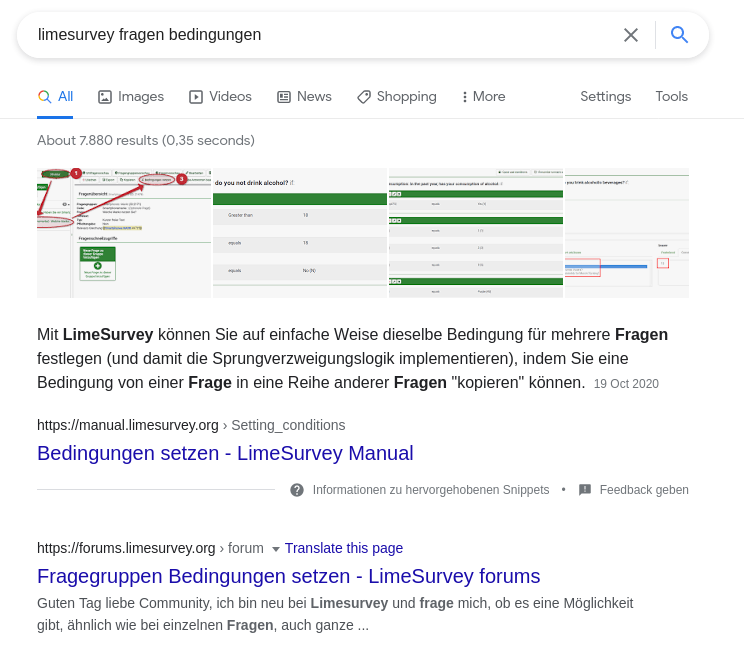
\includegraphics[width=\linewidth]{images/google-search.png}
	\end{columns}
\end{frame}

\begin{frame}{Wenn mal was nicht so klappt wie gewünscht...}
	\begin{block}
		{Langsame Webseite}
		Limesurvey hat die Tendenz, lange Ladezeiten zu haben. Wenn es besonders
		schlimm ist sollte auf mehreren Tabs gleichzeitig gearbeitet werden,
		sodass zum Bespiel während eine Frage geladen wird eine andere schon
		bearbeitet wird.
	\end{block}
	\begin{alertblock}{Aber:}
		Es sollten \alert{niemals} zwei Tabs gleichzeitig zu der selben Frage
		offen sein, da sonst beim speichern in einem Tab die Daten im anderen
		verloren gehen können.
	\end{alertblock}
\end{frame}

\begin{frame}{Weitere Features und Möglichkeiten}
	\section{Weitere Features}
	\label{sec:WeitereFeatures}
	Bisher: Die Umfrage war statisch, alle ProbandInnen sahen die gleichen
	Fragen.
	\\
	Jetzt: Dynamische Umfragen
	\begin{block}{Bedingungen setzen}
		Den Fragen kann eine Bedingung zu gewiesen werden. So können Folgefragen
		elegant eingebaut werden (Siehe auch Bild auf der vorherigen Folie).
		\\
		Dazu kann bei den Fragen eine \textbf{Relevance equation} gesetzt werden:
		\\
		Gibt es eine single choice Frage ``position`` mit durchnummerierten
		Optionen, so kann in einer Folgefrage (oder Fragengruppe) die Relevance
		equation
		\\
		\texttt{position==2}
		\\
		gesetzt werden.
	\end{block}
\end{frame}

\begin{frame}
	{Weitere Features und Möglichkeiten}
	\begin{example}
		Als Beispiel von einer alten Umfrage wo gezielten Folgefrage(-gruppen) an
		Lehrkräfte gestellt wurden:
  	  	\begin{figure}
  	  	      \centering
	  	      \begin{subfigure}[b]{0.4\textwidth}
          			\centering
    	  	      		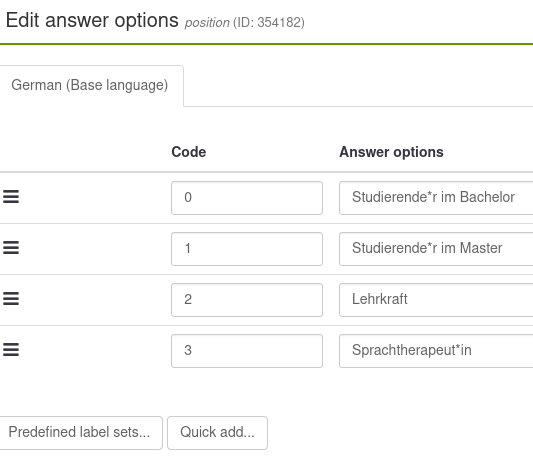
\includegraphics[height=4.5cm]{images/answer-options.png}
				\caption{Antwortmöglichkeiten einer multiple choice Frage,
				Fragencode=``position``.}
	  	      \end{subfigure}
	  	      \begin{subfigure}[b]{0.4\textwidth}
			      \centering
			      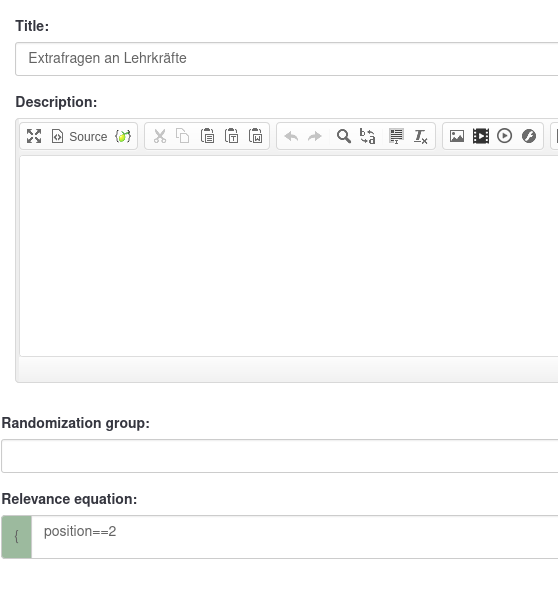
\includegraphics[height=4.5cm]{images/extrafragen.png}
			      \caption{Folgefragengruppe speziell an Lehrkräfte mit
			      Relevance Equation, die ``position`` aufgreift.}
	  	      \end{subfigure}
	  	\end{figure}
	\end{example}
\end{frame}

\begin{frame}
	{Weitere Features und Möglichkeiten}
	Weitere Dynamik: Die Teilnehmenden zufällig in mehrere Gruppen aufteilen
	(\alert{A/B Test})
	\\ \medskip
	\begin{block}{Fragentyp: Equation}
		Der Fragentyp ``Equation`` ist eine Frage, die der \alert{Teilnehmer nicht 
		sehen kann}, sie findet im Hintergrund statt. Die Antwort beruht auf einer
		mathematischen Formel, die frei definiert werden kann.
		\\
		Wichtig sind für uns die Funktionen \texttt{floor()} und \texttt{rand()}:
		\begin{itemize}
			\item \texttt{rand(1,4)} erstellt eine zufällige Zahl zwischen 1
				und 4 (inklusive Rand),
			\item \texttt{floor(x)} Rundet die Zahl x nach unten.
		\end{itemize}
		Theoretisch würde \texttt{floor(x,y)} schon reichen weil es
		(\alert{scheinbar}) nur ganze Zahlen generiert, habe es aber nie getestet.
	\end{block}
\end{frame}

\begin{frame}
	{Weitere Features und Möglichkeiten}
	\begin{figure}
		\centering
		\begin{subfigure}[b]{0.2\textwidth}
			\centering
			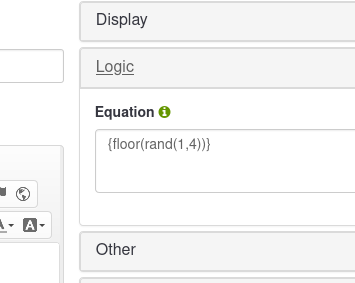
\includegraphics[height=3.5cm]{images/randomizer-equation.png}
			\caption{Deklaration der equation-Frage ``randomizer1``, hier mit
			vier Gruppen.}
		\end{subfigure}
		\begin{subfigure}[b]{0.7\textwidth}
			\centering
			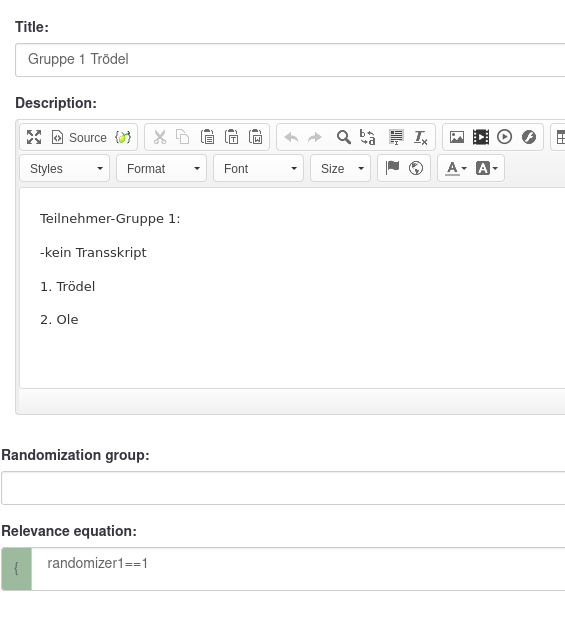
\includegraphics[height=5.5cm]{images/groupe-relevance.png}
			\caption{Aufgreifen des Ranomizers in einer Relevance equation}
		\end{subfigure}
	\end{figure}
\end{frame}

\begin{frame}
	{Weitere Features und Möglichkeiten}
	\begin{alertblock}{Gefahr bei rand()}
		Eine Gefahr ist hier, dass die \texttt{rand(x,y)} Funktion immer neu
		ausgeführt wird, wenn der Teilnehmer die Seite neu aufruft, wenn er zum
		Beispiel wieder zurück geht in der Umfrage.
		\\
		Damit kann er dann zum Teil erst in Gruppe A, dann in Gruppe B sein.
	\end{alertblock}
	\medskip
	Dazu gibt es zwei Lösungen:
	\begin{block}{Quick and dirty solution}
		Die Umfrage sehr früh in die Umfrage stecken und die Gruppenspezifischen
		Inhalte zum Ende.
	\end{block}
	\medskip
	\begin{block}{Saubere Lösung}
		Lime Survey kann überprüfen, ob der random Wert schonmal zugewiesen wurde.
		\\
		Setzt man als Equation
		\begin{center}
			\texttt{if(is\_empty(self), rand(1, 4), self)}
		\end{center}
		so überprüft Limesurvey bei jedem Aufruf, ob schonmal ein randomizer
		zugewiesen wurde.
	\end{block}
\end{frame}

\begin{frame}{Literatur}
	\printbibliography{}
\end{frame}

\end{document}
